%\documentclass[10pt,draft,conference]{IEEEtran}
\documentclass[10pt,final,conference]{article}

\usepackage{amsmath,amsfonts,amssymb,amscd,amsthm,xspace}
\usepackage{algorithm}
\usepackage{algorithmic}
\usepackage{graphicx}
\usepackage{caption}
\usepackage{subcaption}
\usepackage[square, numbers, comma, sort&compress]{natbib}
\usepackage{fancyhdr}
\usepackage{listings}
\usepackage[colorlinks,linkcolor={black},citecolor={blue}, urlcolor=black]{hyperref}

\begin{document}

\title{Final Project: Asteroid Planning}
\author{Robot Intelligence: Planning 4649/7649 \\
Group 2: Kyle Volle, Luke Tornquist, Steffan Slater, Xinyan Yan}
\maketitle

%\tableofcontents{}

\newpage

\nocite{*}

\begin{abstract}
In this paper, planning and machine learning concepts are applied to the design of an autonomous agent to play an "asteroids" type computer game. The game presents unique challenges in limited movement range, spawning of more and smaller asteroids after a bullet impact, and elastic asteroid-asteroid interactions. Two components of the game are investigated - selecting a direction in which to move the craft and selecting a direction in which to fire bullets in an attempt to destroy asteroids and increase the score. A velocity obstacle approach is used to determine safe directions for the craft to travel, and one of those safe headings is selected in one of several manners.
\end{abstract}

\section{Member Responsibilities}
For this project, Kyle was in charge of writing the introduction and putting together the results and plotting the data, both in the paper as well as in the presentation.  Luke developed the Asteroids game, and created the remote interface for the planner to utilize.  Luke also worked on the decision tree algorithm that is utilized in calculating when the ship should fire and when it should not.  He also typed up the relevant sections in the paper and put together the video for the presentation.  Steffan wrote all of the Navigation planning algorithm, which does almost all of the motion planning for the ship.  He also did a significant amount of research regarding the planning algorithms that have been historically associated with the asteroids problem.  He also typed up all his relevant parts in the paper, and presentation.  Xinyan worked on creating the motion planning machine learning, that was to be used for helping determine which "safe" heading to choose when multiple are present.  Due to time constraints and other unforseen circumstances, the motion planning machine learning was not completed, but instead Xinyan completed the Preview planning algorithm.  Xinyan also worked on typing up his relevant parts in the paper and presentation.

\section{Introduction}
The "asteroids" genre of games poses several interesting planning problems. In this game, the player controls a spaceship in an environment that is filled with fast moving obstacles called asteroids. Collision with an asteroid causes the player to lose a life. Points are scored by shooting the asteroids and breaking them into two smaller, faster obstacles. Asteroids progress from large to medium to small. If a small asteroid is hit, it is removed from the game. As the game goes on more and more obstacles are spawned. The goal for the player then is to stay alive as long as possible to keep shooting asteroids.

This game is interesting for several reasons. For starters there is no final goal, but rather the planner seeks to stay alive for as long as possible. This differentiates this problem from more traditional motion planning problems. Additionally, in this game there are no static states. Conservation of momentum keeps the ship moving at a constant velocity if there is no player input. Combined with the dynamic nature of the obstacles, the game state can change rapidly requiring frequent replanning.

The planner utilizes several processes in order to maximize the potential future score. An array of safe trajectories is first calculated and from this list another process selects one of these trajectories based on the anticipated rewards and costs. Finally, a third process determines the game inputs corresponding to following this trajectory and places these inputs in an executor queue to be performed as the replanning occurs. Factors for selecting a trajectory include, but are not limited to, time required to achieve that trajectory, density of asteroids along the trajectory, distance to obstacles along the trajectory and the ability to destroy asteroids along the way. The Methods section will go into greater detail about the techniques and strategies employed.

\section{Related Work}

A significant amount of literature exists for the problem of navigation with mobile obstacles. This literature tends to fall into one of two categories - local methods or global methods, based on how obstacles influence robot behavior \cite{khansari2012dynamical}. Local methods include bug algorithms and the Vector Field Histogram, while global methods include artifical potential fields and visibility graphs. Local methods tend to run rapidly but may not find feasible paths, while global methods will find a valid solution if there is one but tend to be slow. Given that our environment can be frequently changing as asteroids collide or are struck by bullets and break apart, a local method would appear to be a better choice to allow for rapid replanning; however, including some ability to look ahead is critical in an environment with moving obstacles. 

The selected approach for navigation planning is based on the concept of velocity obstacles, which takes into account all future obstacle/robot future relative positions, assuming constant velocities \cite{fiorini1998motion}. The constant velocity assumption is acceptable for our problem as the plan will be rebuilt frequently, which will account for any asteroid-asteroid or asteroid-bullet interactions. While the exact approach used will be described in detail later, the concept is to convert the space and time domain into a purely spatial representation which can be easily searched for collisions. This results in a velocity space representation of the robot and obstacles, which is then used for planning. This approach, unlike some navigation methods, generalizes well to real-world applications of robots with limited sensors and domain knowledge, and has been used for autonomous surface vessel navigation in the crowded Singapore harbor \cite{bandyophadyay2010simple}. 

\section{Methods}

\subsection{Game Development}
We decided to develop the game ourselves due to the lack of open source projects that had all the functionality that we desired.  We utilized LibGDX as the basic framework for creating the game.  LibGDX is built on Java, so we decided to use Java for the planner as well.  The game mechanic that we really wanted in our game was to have realistic physics in regard to collisions.  Most open source games out there do not have this feature, as the original Asteroids game did not have it either.  We added this functionality using the Box2D libraries that come built in to LibGDX.  This allowed us to give asteroid collisions a more realistic feel, and it also made the game a good bit more difficult.  Another very important reason that we chose to develop the game ourselves was the fact that it allowed us to get access to any data that we needed from the game.  We created all of the entities (Ship/Asteroids) as circular objects to simplify our calculations.  The textures that we used, also seemed to be that way, so it fit well.

\subsection{Game and Planner Interface}
The planner interfaces with the game using Remote Method Invocation (RMI).  This method of remote calls is supported in Java to allow interprocess communication.  This is how we transfer game data from the game to the planner, as well as transfer plan actions from the planner to the game.  The way it works is pretty basic as it functions much like a client/server model.  The Game functions as the RMI Server and registers with the local RMI Registry to expose the interface to other processes.  The Planner functions as the RMI Client and queries the RMI Registry for the exposed interface.  This returns as shared object that allows the planner to call any exposed methods remotely.

\subsection{Navigation Planning}

The navigation planning approach is based upon the velocity obstacle method described in \cite{fiorini1998motion}. The motion of the robot and a single obstacle is transformed into relative motion of the robot and a stationary obstacle at the same current position. The asteroid is then expanded by the radius of the robot plus a safety factor. This safety factor prevents this method from being complete, as it can cause the planner to miss potential feasible passages, but compensates for inaccuracies in the turning maneuvers and the slight lag of the planner behind the actual game execution. This expansion of the asteroid collapses the spacecraft to a point, moving the problem into the more tractable configuration space. 

After expanding the asteroid, the exclusion cone of the obstacle is computed. This cone consists of two rays from the current robot position through the tangency points of the obstacle. Since the velocity obstacle approach transforms a moving obstacle to a stationary one, any robot velocity relative to the obstacle which falls into the exclusion cone will at some point result in a collision. The current relative velocity of the robot to the obstacle is then placed in the space, and may or may not be within the exclusion cone of the obstacle. It is then necessary to compute the range of possible relative velocities after some amount of time.

The computation of the possible relative velocities is accomplished by computing the potential change in velocity in each direction based on the robot's current attitude. In Asteroids this presents an interesting problem, as the space of potential velocity changes is not a simple shape. While a two-degree-of-freedom actuated effector such as the print head on a 3D printer has a rectangular velocity change space (as the two directions are independent), and a vehicle which can apply a thrust linearly in any direction has a circular velocity change space, the craft in Asteroids can only accelerate forward and has a finite turn speed. This means that for a given amount of time, the craft can accumulate more change in velocity in a forward direction than in any other direction, as it must first turn before accelerating in that direction. This results in a heart-shaped velocity change space given by the equation:

\begin{equation*}
\Delta v(\theta) = a \left( \Delta t - \frac{\theta}{\omega} \right)
\end{equation*}

where $a$ is the acceleration of the craft and $\omega$ is the angular velocity while turning. This velocity change space is then rotated by the craft attitude and translated by the relative velocity to obtain the set of reachable relative velocities within the time step. The time step used is the time required to perform a 180-degree turn and accelerate to 25\% of the ship maximum velocity or the shortest time to impact, whichever is smaller. 

The set of reachable relative velocities is then intersected with the exclusion cone to find which directions (headings) are safe for the craft to move along. This is done by calculating the angle from the current position to each point on the reachable velocity curve and searching for all points where that angle is equal to the angle of the edges of the exclusion cone, as those tangent lines are lines of constant angle (radial lines in polar coordinates). Which side of the intersection heading is safe is determined by picking a point on either side and taking the sum of the angles between the tangent lines and a line though the current position and that point. If the sum is equal to the angle between the two tangent lines, it is between the two and therefore in the exclusion zone. If that sum is greater than angle between the two tangents, it is outside the exclusion zone. This strategy will give the safe and unsafe heading ranges for the craft based on a single obstacle. The results for all obstacles can then be superimposed to get the overall safe and unsafe ranges. An example of a reachable velocity region with an exclusion cone is shown in Figure \ref{fig:reachable_veloc}, with the relative velocity in blue, the axis of the craft in dashed black, the reachable velocities in solid black, and the boundaries of the exclusion cone in red.

\begin{figure}[ht]
\centering
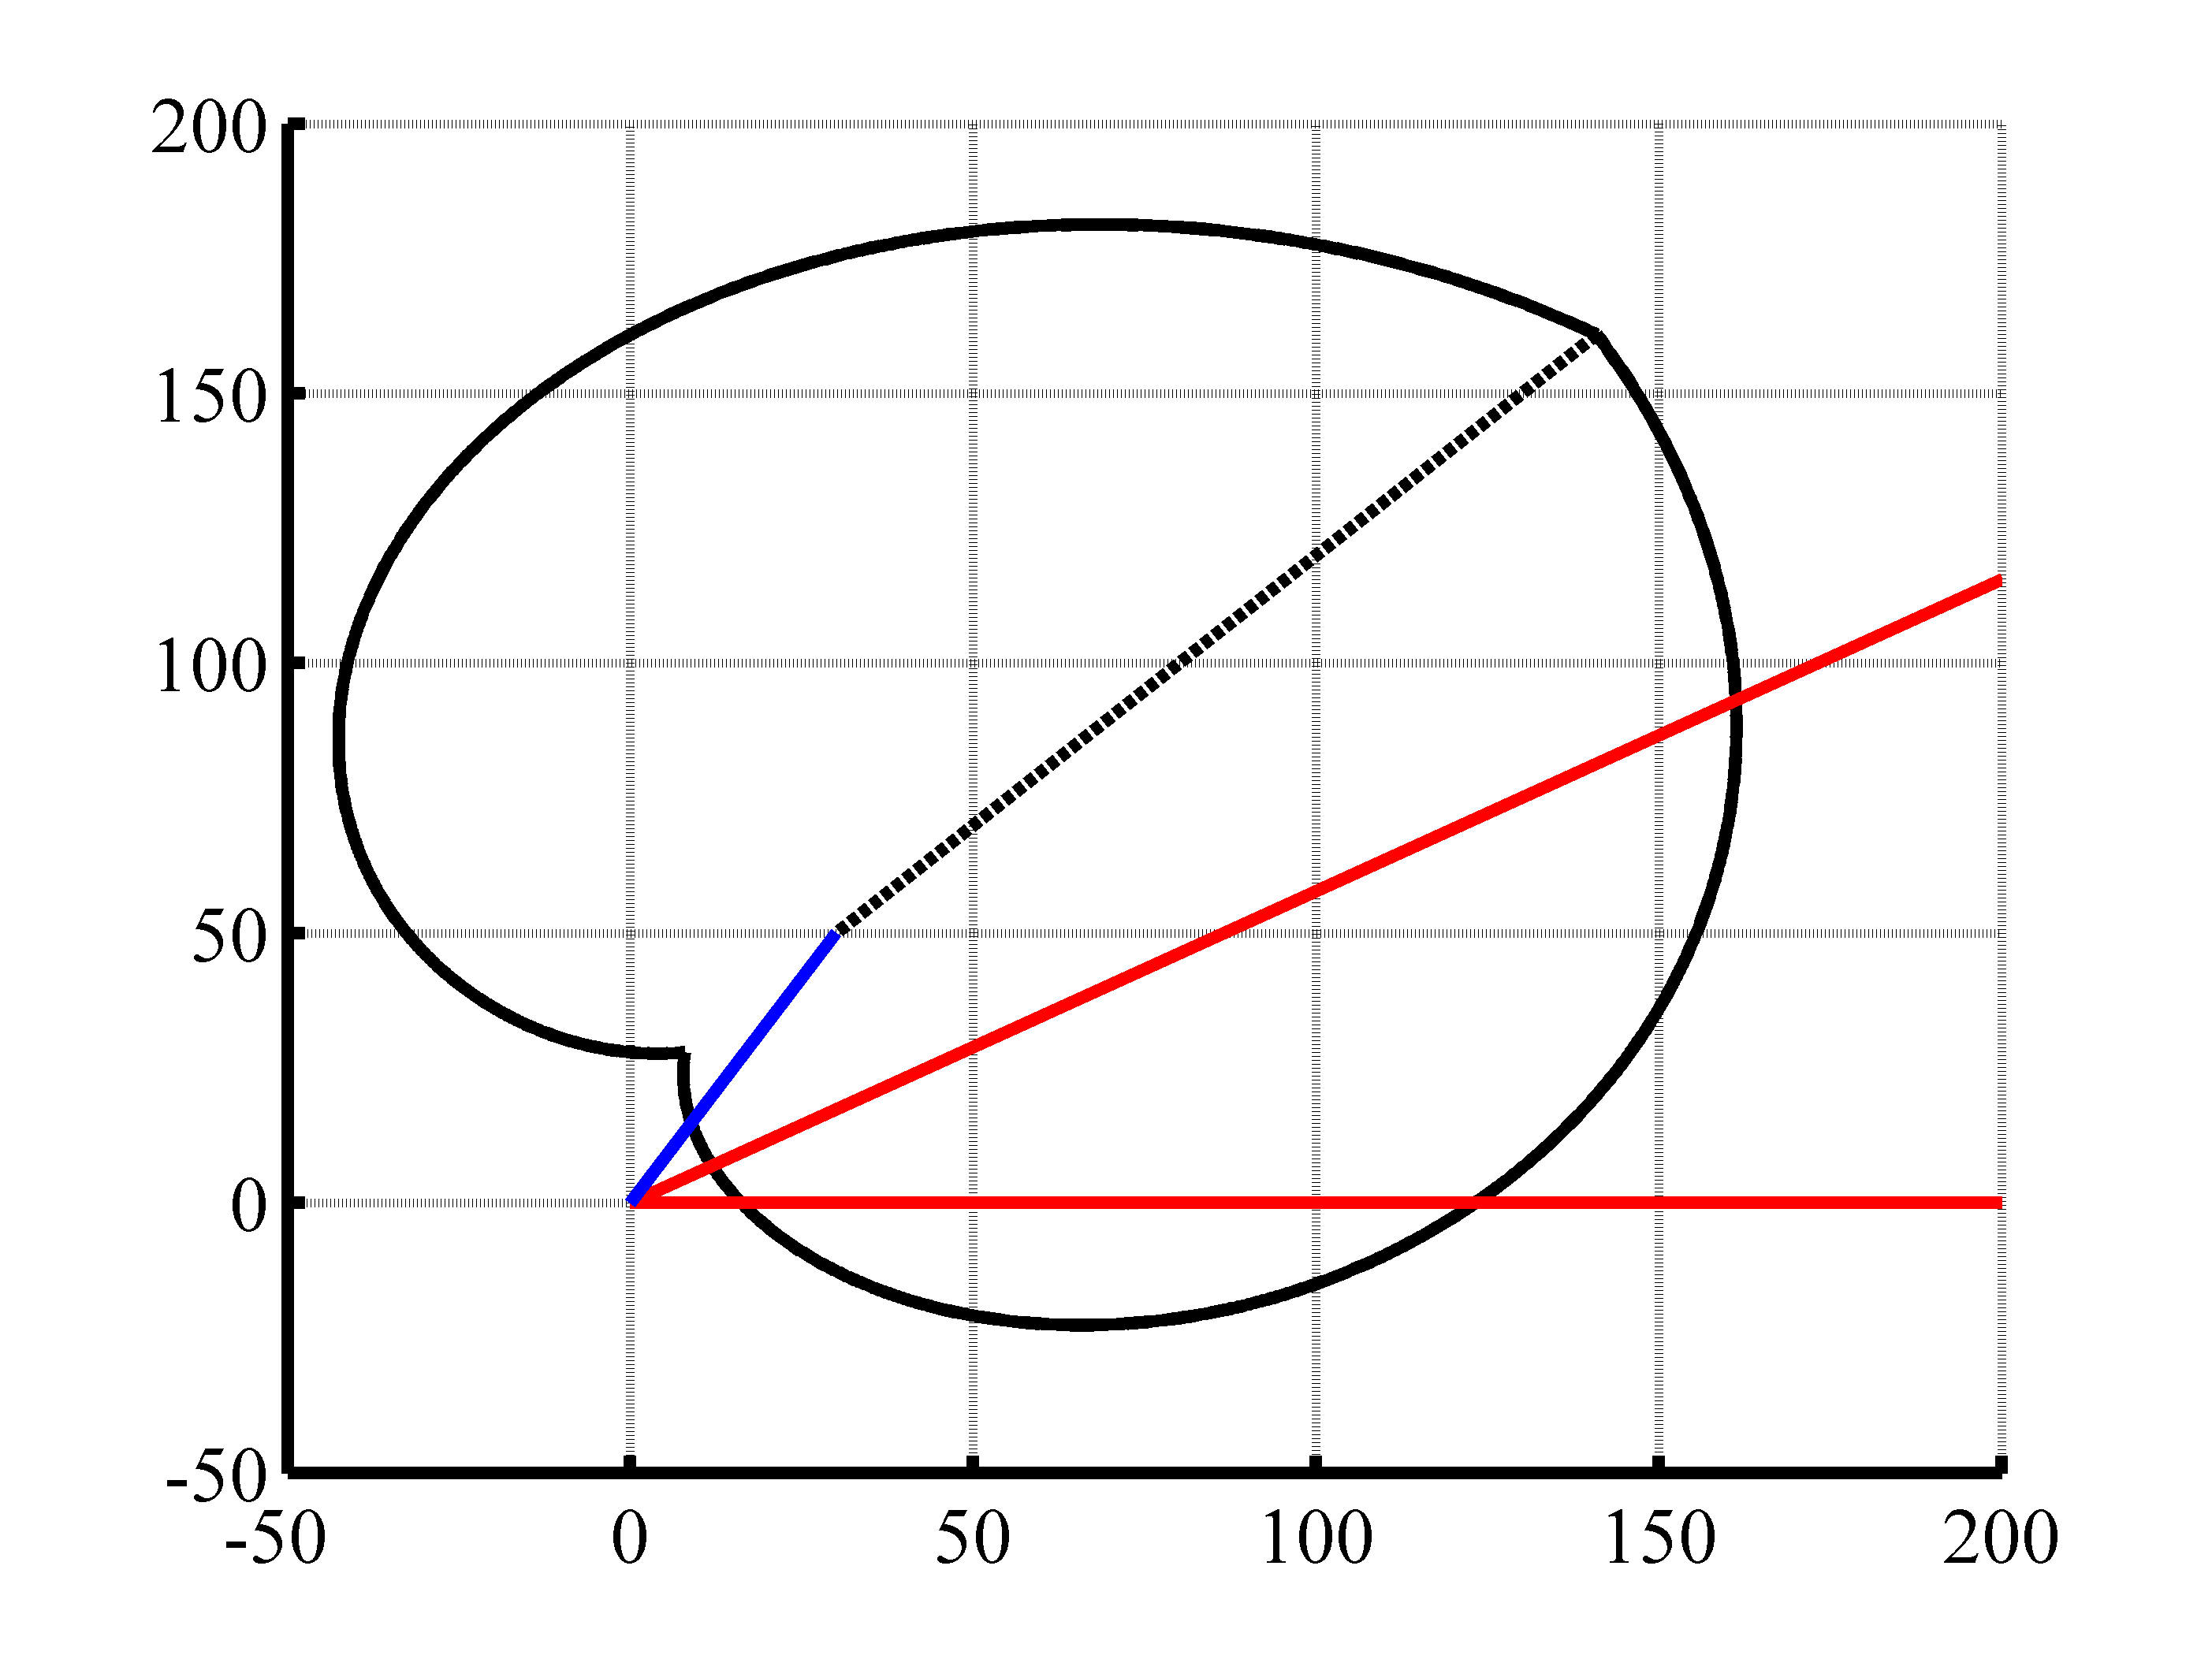
\includegraphics[width=3in]{./deltav_curve_rotated_translated_obstacle_color.png}
\caption{Reachable Velocities with Exclusion Cone}
\label{fig:reachable_veloc}
\end{figure}

To ensure that not all headings are excluded, only asteroids within some distance of the craft are considered. This distance can be modified by the planner, for example by reducing the search radius to open up more safe headings. From the set of safe headings, one heading is selected as the target and a rotation and acceleration maneuver to that heading is computed. The selection of the heading is the true job of the navigation planner. Most of the extant literature focuses on using the velocity obstacle approach to calculate a path to a goal point, but Asteroids does not have a goal point. The selection of the target heading must therefore be chosen in a different manner. One method that was considered, for example, was selecting the safe heading closest to the current direction, thereby minimizing the amount of turning that was to be carried out.

\subsection{Decision Trees}
Decision trees were used to predict whether we should or should not shoot at each particular asteroid.  We used decision trees as they allow us to classify particular situations based on a set of input variables, and learn from success and failure to learn over time.  This should allow the ship to get more adapt at figuring out when it is good to fire and when it is not.  The output of the tree is basically a classification for that particular set of variables in the tree, which correlates to the path from the leaf node to the root of the tree.  That classification maps to either true or false in our case, as we are trying to decide whether we should fire or not.

\begin{figure}
\centering
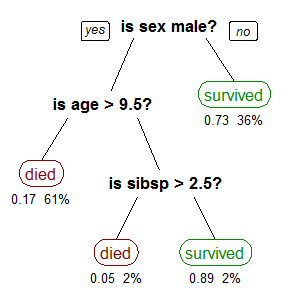
\includegraphics[width=3.0in]{./CART_tree_titanic_survivors.png}
\caption{Decision Tree - Example\cite{titanic}}
\label{fig_decision_tree_example}
\end{figure}

Figure [\ref{fig_decision_tree_example}] is an example decision tree that was used as a basis for the decision tree creation for the Asteroid Planner\cite{wikiDecisionTreeLearning}.  It was used as an example because we needed to persist a similar kind of data, which is basically a numeric value which corresponds to the success rate of firing mapping to a successful outcome.  This numeric value is then used to predict whether we should fire or not.  Similar metrics are used in Figure [\ref{fig_decision_tree_example}] except the outcomes are died or survived.

\begin{figure}
\centering
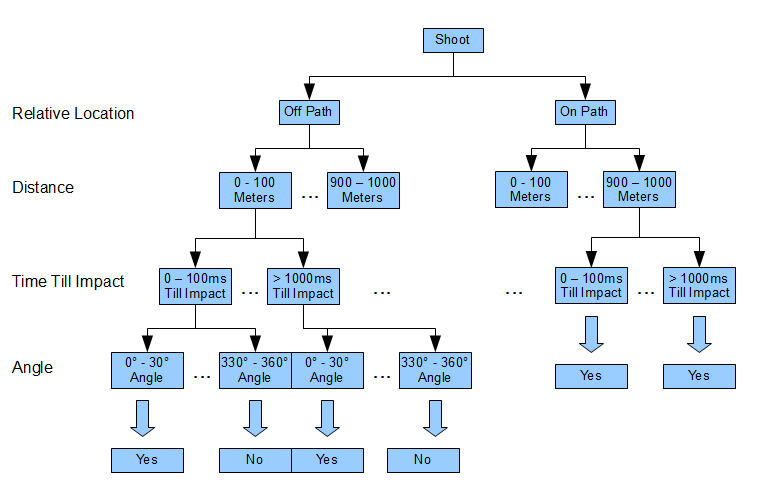
\includegraphics[width=3.0in]{./DecisionTree.png}
\caption{Decision Tree - Asteroids Planner}
\label{fig_decision_tree_asteroids}
\end{figure}

Figure [\ref{fig_decision_tree_asteroids}] is the layout of our decision tree that we utilized for fire planning in our system.  We used a few metrics that would help classify every asteroid each time we analyzed it.  The first metric was relative path, and it was simply a true or false value that was true if the asteroid could cross our line of sight as we avoided any obstacles, and false otherwise.  The next metric is the distance that the asteroid is from the ship, which can obviously be a very helpful metric.  Another metric we decided to use was the time till impact.  This takes into account not only the distance of the asteroid, but also the velocity of that asteroid.  Finally, the last metric we decided to use was the angle that the asteroid was from our current ship heading.  Since some of these metrics were numeric, rather than boolean, we decided to segment each of the metrics into ranges, and use those as a more granular way to classify the asteroids.  In Figure [\ref{fig_decision_tree_asteroids}] you can see the ellipsis' between the nodes that have ranges, because they are there to represent the numerous nodes that would exist between the two nodes.

At each leaf, we keep a few pieces of vital information that we use to determine the usefulness of the data as well as the predictability.  

\subsection{Preview Planning}
Navigation planning provides a range of plausible headings to take. However, which heading is the best one to pick? Here, the previewer comes to play. Basically, it outputs the action which leads to an optimal action sequence. It is optimal in terms of the sum of discounted rewards n steps into the future.

When we are making decisions, definitely we take the results of actions into account, for example, whether we will be in good state or not after taking one action. Sometimes, we think further into the future. For example, when players are playing chess, the better they are, the farther into the future they will consider the impact of the current step. Applying this to asteroid planning, in order to choose a good heading from a pool of plausible headings, we consider heading samples as possible actions to choose. High reward can be achieved if the resulted state looks good, and the turn angle is small. 
\begin{equation} \nonumber
\begin{split}
\text{States\ \ \ \ }\ &\sum = \{s_1,..., s_n\}  \text{\ \ \ \ consist of angle, position and velocity of the ship and asteroids} \\
\text{Actions\ \ \ \ }\; &A = \{a_1,..., a_n\} \text{\ \ \ \ \ \ represent different headings} \\
\text{Rewards\ \ \ \ }\; &R = \{r(s_i, a_j)\} \text{\ \ \ \ \ \ \ reward we'll get if we take action $a_j$ in state $s_i$}
\end{split}
\end{equation}
The optimal action $\hat{a}$ to take in state $s_i$ would be:
\begin{equation} \nonumber
\begin{split}
\hat{a} = \arg\max_{a} \left ( r(s_i, a) + \gamma r(s_j, a_m) + \gamma^2 r(s_k, a_n) + ... + \gamma^{n-1} r(s_l, a_o) \right ) 
\end{split}
\end{equation}
In the equation, $s_i \rightarrow s_j \rightarrow s_k \rightarrow ... \rightarrow  s_l$ is a sequence of states.
Because the dynamics of asteroids and ships are totally deterministic, and we know the state exactly by reading game data, we don't have any execution error or sensing error, which makes preview planning very simple. Although we do have uncertainty about where new asteroids will be created at what velocity, we neglect it because of its high complexity and small impact. To solve this problem, we build a tree, in which nodes denote states and edges denote actions associated with discounted rewards. We trace back the tree to find a maximal path. Then we choose the first action in the path to take. 

\section{Experiments}

In the experiment, we tried different parameters. And we found several influential parameters. They are: (1) running frequency of planner, (2) number of steps taken into account, and (3) penalty for large turn angles. Because the ship needs relative quick reaction, and the number of nodes of the tree increase exponentially with the horizon which take much more time to compute the best path, horizon = 1, running frequency = 200ms, turning penalty = 0.1 are the best parameter combination we got so far. 


\section{Analysis}


\section{Discussion}


\bibliography{Reference}
\bibliographystyle{unsrtnat}

\end{document}